% !TEX root = ../main.tex
\section{Free-rider-problemet (nedstrøms)}\label{thr:free-rider-problem}

\paragraph{Definisjon.} I konteksten vertikal integrasjon vs.\ outsourcing oppstår \emph{free-rider-problemet} når uavhengige distributører underinvesterer i aktiviteter som gagner merket/produktet som helhet (service, markedsføring, showroom), fordi gevinsten av deres innsats deles med -- eller fanges av -- andre distributører. [SLIDE]

\subsection*{Forklaring}

BSZ kap.\ 19 diskuterer free-riding som et sentralt kontraktproblem ved outsourcet distribusjon. [SLIDE/BOK]

\textbf{Mekanisme:}
\begin{enumerate}\setlength{\itemsep}{2pt}
\item Produsent $P$ selger via uavhengige distributører $D_1, D_2, \ldots, D_n$.
\item Investering i kundeservice, showroom, rådgivning og lokal markedsføring er kostbart for den enkelte distributør.
\item Kunden bruker $D_1$s showroom for å teste produktet, men kjøper billigere fra $D_2$ som ikke investerer i service (\emph{inter-dealer free-riding}).
\item $D_1$s investering skaper en \emph{positiv eksternalitet} for $D_2$ -- en form for \thref{externalities}{eksternalitet} som markedet ikke internaliserer.
\item \emph{Resultat:} Alle distributører underinvesterer i service, merkevareverdi eroderes, og produsenten taper.
\end{enumerate}

\textbf{Varianter:}
\begin{itemize}\setlength{\itemsep}{1pt}
\item \textbf{Service free-riding:} Kunde bruker high-service dealer for rådgivning, kjøper fra discounter.
\item \textbf{Brand free-riding:} Distributør leverer dårlig service, men nyter godt av produsentens merkevare.
\item \textbf{Advertising free-riding:} Én distributørs reklamekampanje trekker kunder til regionen, men konkurrerende forhandlere fanger salget.
\end{itemize}

\textbf{Løsninger:}
\begin{itemize}\setlength{\itemsep}{2pt}
\item \textbf{Vertikal integrasjon} -- produsenten eier distributørkjeden og internaliserer eksternaliteten. [SLIDE]
\item \textbf{Resale price maintenance (RPM):} Minimumspris forhindrer priskutt som undergraver service-insentiv. Kontroversielt pga.\ konkurranserett. [BOK]
\item \textbf{Eksklusive territorier:} Hver distributør har monopol i sitt geografiske område -- inter-dealer free-riding elimineres. [BOK]
\item \textbf{Franchising med standardiserte servicekrav:} Franchisetaker forpliktes kontraktuelt til å investere i service (McDonald's, BMW). Brudd gir oppsigelse av kontrakt. [SLIDE]
\item \textbf{Produsenten finansierer:} Sentralisert markedsføring/service (co-op advertising) betalt av produsenten, fordelt via avgift. [BOK]
\end{itemize}

\subsection*{Kjerneforutsetninger}
\begin{itemize}
\item Distributørens serviceinvestering skaper verdi for kunder som kan kjøpe \emph{andre steder}.
\item Kunden kan separere informasjonsinnhenting fra kjøp (showrooming).
\item Distributørene er uavhengige profittmaksimerende enheter.
\item Produsenten kan ikke gratis observere eller kontrollere servicenivå (\thref{moral-hazard}{moral hazard}).
\end{itemize}

\subsection*{Muligheter}
\begin{itemize}
\item Forklarer franchising-modellens logikk: standardiserte kvalitetskrav + insentivsystem.
\item Forklarer eksklusive forhandleravtaler, minimumsannonsering og servicekrav i bilbransjen.
\item Forklarer hvorfor luksusmerker kontrollerer distribusjon strengere enn massemerker.
\end{itemize}

\subsection*{Begrensninger og kritikk}
\begin{itemize}
\item Internett har gjort showrooming massivt -- løsningene (RPM, eksklusive territorier) er stadig vanskeligere å håndheve.
\item RPM og eksklusive territorier kan være kartell-/monopolverktøy forkledd som anti-free-riding.
\item Franchising-kontrakten er selv kostbar å håndheve (\thref{costly-contracting}{costly contracting}).
\item Noen produkter trenger lite pre-sale service -- free-riding er da irrelevant, og outsourcing er uproblematisk.
\end{itemize}

\subsection*{Modell / illustrasjon}

\begin{figure}[H]
  \centering
  
\includegraphics[width=0.45\linewidth]{BSZ_kap_9_2026/by_slide/slide_015/BSZ_kap_9_2026_slide_015_asset_01_image4.jpeg}
  \caption{Free-rider-problemet i hverdagen: oppvasken ingen tar -- alle nyter godt av et rent kjøkken, men ingen vil bære kostnaden alene. (BSZ kap.\ 9, slide 15) [SLIDE]}
\end{figure}

\begin{center}
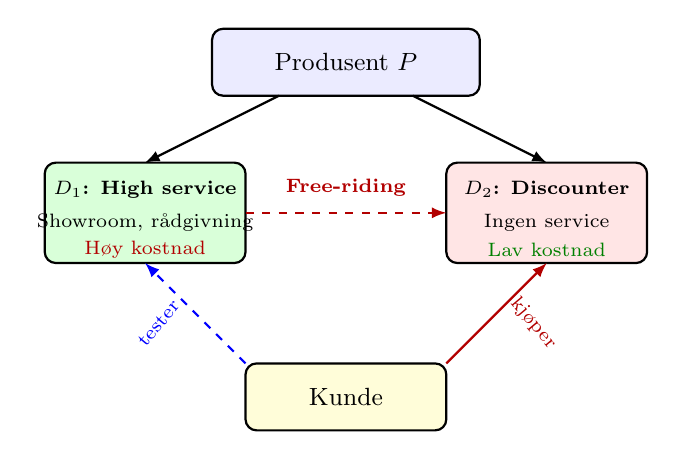
\begin{tikzpicture}[>=latex, scale=0.85, every node/.style={font=\small}]
  % Produsent
  \draw[thick, rounded corners, fill=blue!8] (3,5.5) rectangle (7,6.5);
  \node at (5,6.0) {Produsent $P$};
  % D1 high service
  \draw[thick, rounded corners, fill=green!15] (0.5,3.0) rectangle (3.5,4.5);
  \node[font=\bfseries\scriptsize] at (2,4.1) {$D_1$: High service};
  \node[font=\scriptsize] at (2,3.6) {Showroom, rådgivning};
  \node[font=\scriptsize, red!70!black] at (2,3.2) {Høy kostnad};
  % D2 discounter
  \draw[thick, rounded corners, fill=red!10] (6.5,3.0) rectangle (9.5,4.5);
  \node[font=\bfseries\scriptsize] at (8,4.1) {$D_2$: Discounter};
  \node[font=\scriptsize] at (8,3.6) {Ingen service};
  \node[font=\scriptsize, green!50!black] at (8,3.2) {Lav kostnad};
  % Arrows from P
  \draw[->, thick] (4,5.5) -- (2,4.5);
  \draw[->, thick] (6,5.5) -- (8,4.5);
  % Kunde
  \draw[thick, rounded corners, fill=yellow!15] (3.5,0.5) rectangle (6.5,1.5);
  \node at (5,1.0) {Kunde};
  % Kunde besøker D1, kjøper hos D2
  \draw[->, thick, dashed, blue] (3.5,1.5) -- (2,3.0);
  \node[font=\scriptsize, blue, rotate=50] at (2.2,2.1) {tester};
  \draw[->, thick, red!70!black] (6.5,1.5) -- (8,3.0);
  \node[font=\scriptsize, red!70!black, rotate=-50] at (7.8,2.1) {kjøper};
  % Free-rider label
  \draw[->, thick, red!70!black, dashed] (3.5,3.75) -- (6.5,3.75);
  \node[above, font=\scriptsize\bfseries, red!70!black] at (5,3.85) {Free-riding};
\end{tikzpicture}
\end{center}
\textit{Figur: Free-rider-problemet. Kunden tester hos high-service $D_1$ men kjøper hos discounter $D_2$. $D_2$ free-rider på $D_1$s service-investering. Begge distributører underinvesterer i likevekt. [BOK]}

\subsection*{Eksempler}
\begin{itemize}\setlength{\itemsep}{2pt}
\item \textbf{BMW og autoriserte forhandlere.} BMW krever at forhandlere investerer i showroom-standard, opplært personale og verkstedkvalitet. Uten disse kravene ville billige ``broker''-forhandlere free-ride på BMWs merkevare og autoriserte forhandleres serviceinvestering. Løsning: franchising med strenge standarder og eksklusive territorier. [EKS]
\item \textbf{Amazon vs.\ fysiske bokhandlere.} Bokhandlere med rådgivning og events investerer i leseropplevelse, men kunder scanner ISBN og bestiller billigere på Amazon (\emph{showrooming}). Klassisk free-riding -- har bidratt til nedleggelse av bokhandlere globalt. [EKS]
\item \textbf{Mærsk og agenter i utviklingsland.} Mærsk bruker egne kontorer i noen markeder (integrert) og uavhengige agenter i andre. Agenter kan underinvestere i Mærsk-spesifikk kundeservice fordi de også selger for konkurrenter -- free-riding på Mærsks merkenavn. [CASE]
\end{itemize}

\subsection*{Kobling til søyle og andre teorier}
Søyle: \SThree\ (insentivdesign for distributører) og \SOne\ (kontroll via eierskap eller kontraktsvilkår). Relaterte: \thref{vertical-integration-outsourcing}{Vertikal integrasjon og outsourcing}, \thref{externalities}{Eksternaliteter}, \thref{moral-hazard}{Moral hazard} (distributørens skjulte handling), \thref{costly-contracting}{Costly contracting}, \thref{residual-claimants}{Residual claimants}.

\paragraph{Brukt i spørsmål:} Q12 (primært), Q11 (referert).
